\subsubsection{Bioacoustic Index Visualization}
For the Bioacoustic index, the value output by the algorithms is an area value under a curve for both the left and right channels where relevant. Thus initially, the best representation of this index would be a stacked area graph, with both the left and right channels included.\\

\begin{center}
	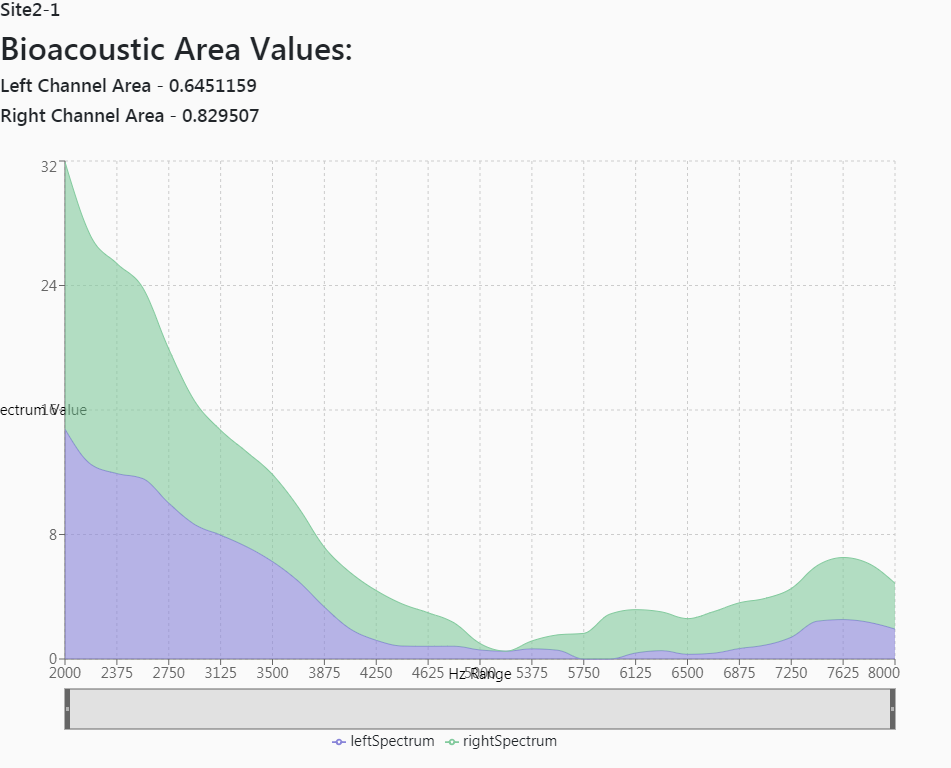
\includegraphics[width=\textwidth]{BAgraph1} \\[12pt]
\end{center}
This graph includes both channels, with a brush included much like in ACI. Because the index calculates a literal area under a curve, an area chart is logically the best representation, and the graphic helps to support this. Again, the user can filter by hertz range using the brush, giving insight into the values in specific ranges. Upon further testing though, it turned out that this particular stacked area graph was not a good way to represent the channels, as their values were not dependent on each other. Thus the following graphs were finalized.\\

\begin{center}
	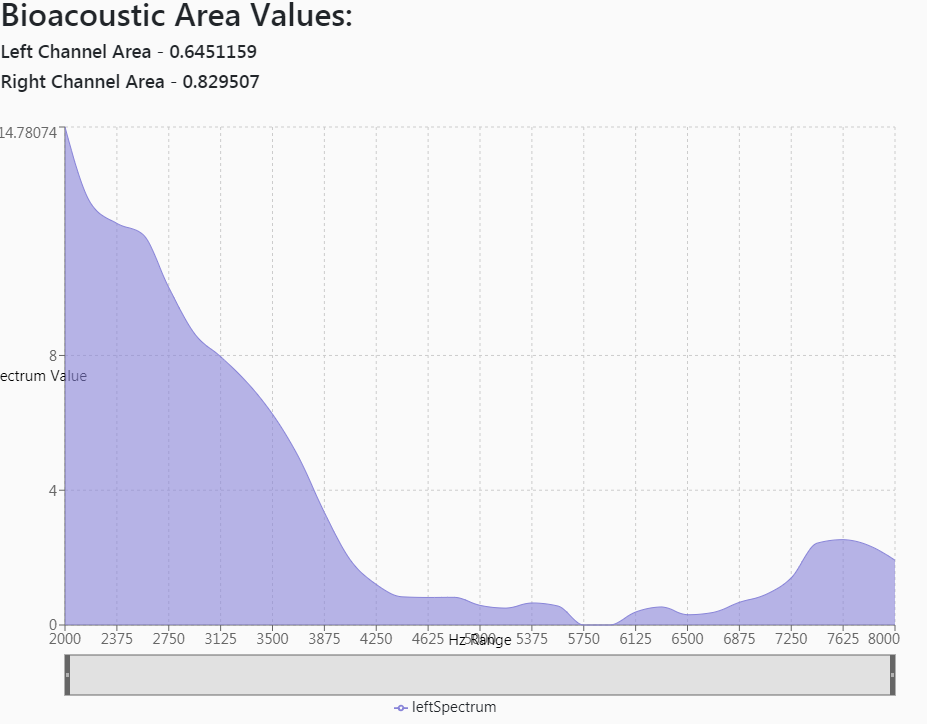
\includegraphics[width=\textwidth]{BAgraph2-1} \\[12pt]
	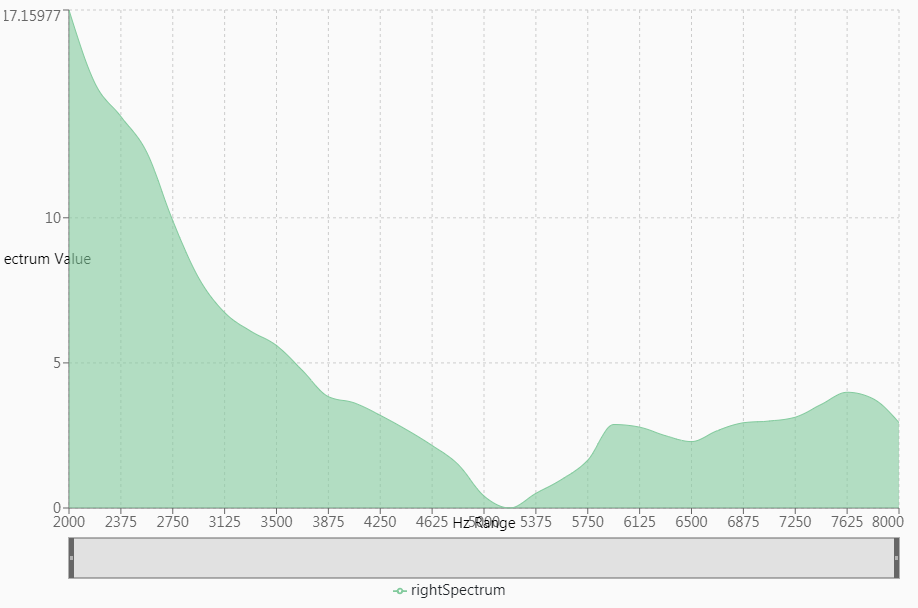
\includegraphics[width=\textwidth]{BAgraph2-2} \\[12pt]
\end{center}

These are a much better representations of the channel areas, as they are no longer dependent on each other as in the last iteration.
